
C++20 is the next big C++ standard after C++11. Like C++11, C++20 changes the way we program in modern C++. This change mainly results from the addition of Concepts, Modules, Ranges, and Coroutines to the language. To understand this next big step in the evolution of C++, let me write a few words about the historical context of C++20.

\begin{center}
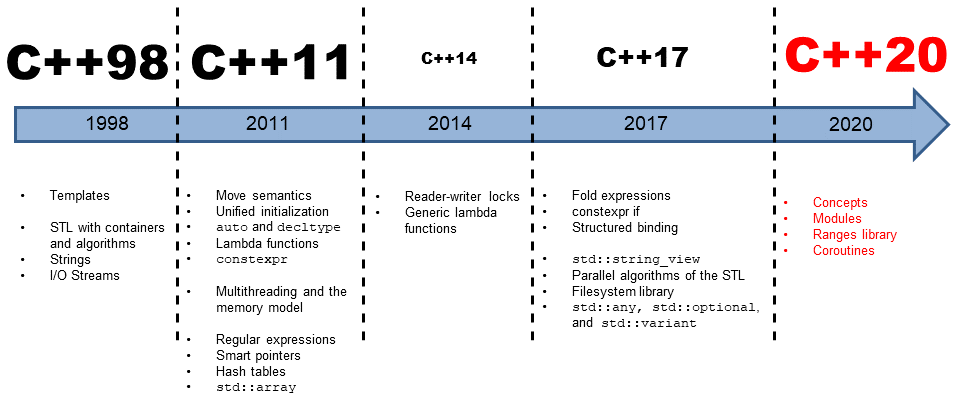
\includegraphics[width=1.0\textwidth]{content/1/chapter1/images/1.png}\\
C++ History
\end{center}

C++ is about 40 years old. Here is a brief overview of what has changed in the previous years.





























